\section{Implementação {\it bottom-up}}

\begin{frame}[fragile]{Número total de nós}

    \begin{itemize}
        \item Suponha que $N = 2^k$, para algum $k$ positivo

        \item Assim, o nível $i$ da árvore terá $2^i$ nós que representam um intervalo de tamanho
            $N/2^i$

        \item A altura $h$ da árvore é igual a $h = \log N = \log 2^k = k$

        \item Logo, o total de nós da árvore será igual a
        \[
            \sum_{i = 0}^k 2^i = 1 + 2 + \ldots + 2^k = 2^{k + 1} - 1 < 2^{k + 1} = 2N
        \]

        \item Assim, a árvore de segmentos deve reservar espaço para $2N$ nós

    \end{itemize}

\end{frame}

\begin{frame}[fragile]{Construtor}

    \begin{itemize}
        \item Em um implementação \textit{bottom-up}, os nós da árvore de segmentos são armazenados
            em um vetor $ns$ de $2N$ elementos, do mesmo tipo dos elementos de $xs$

        \item A posição 0 (zero) não é utilizada, sendo a raiz armazenada no índice 1 (um)

        \item Seja $u$ o nó que ocupa o índice $i$ de $ns$

        \item O filho a esquerda de $u$ ocupará o índice $2i$, e o filho à direita o índice $2i + 1$

        \item O pai de $u$ ocupará o índice $\lfloor i/2\rfloor$

        \item Os elementos de $xs$ ocuparam os índices de $N$ até $2N - 1$

        \item Das folhas até a raiz, um nível por vez, serão preenchidos os nós internos, usando
            a operação subjacente
    \end{itemize}

\end{frame}

\begin{frame}[fragile]{Visualização do construtor da árvore de segmentos}

    \begin{figure}
        \centering

        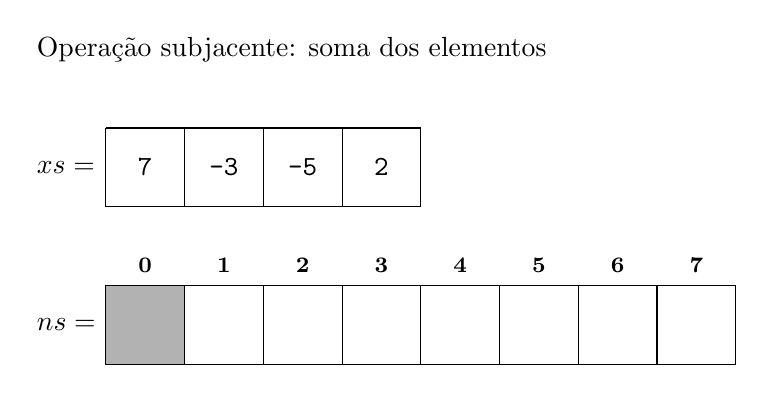
\begin{tikzpicture}
            \node[anchor=west] at (0, 5) { Operação subjacente: soma dos elementos };
            \node[anchor=west] at (0, 3.5) { $xs =$ };
            \node[anchor=west] at (0, 1.5) { $ns =$ };

            \draw[fill=gray!60] (1, 1) rectangle (2, 2);
            \draw (1, 3) grid (5, 4);
            \draw (1, 1) grid (9, 2);

            \node at (1.5, 2.25) { \footnotesize $\mathtt{\mathbf{0}}$ };
            \node at (2.5, 2.25) { \footnotesize $\mathtt{\mathbf{1}}$ };
            \node at (3.5, 2.25) { \footnotesize $\mathtt{\mathbf{2}}$ };
            \node at (4.5, 2.25) { \footnotesize $\mathtt{\mathbf{3}}$ };
            \node at (5.5, 2.25) { \footnotesize $\mathtt{\mathbf{4}}$ };
            \node at (6.5, 2.25) { \footnotesize $\mathtt{\mathbf{5}}$ };
            \node at (7.5, 2.25) { \footnotesize $\mathtt{\mathbf{6}}$ };
            \node at (8.5, 2.25) { \footnotesize $\mathtt{\mathbf{7}}$ };

            \node at (1.5, 3.5) { \tt 7 };
            \node at (2.5, 3.5) { \tt -3 };
            \node at (3.5, 3.5) { \tt -5 };
            \node at (4.5, 3.5) { \tt 2 };
        \end{tikzpicture}
    \end{figure}

\end{frame}

\begin{frame}[fragile]{Visualização do construtor da árvore de segmentos}

    \begin{figure}
        \centering

        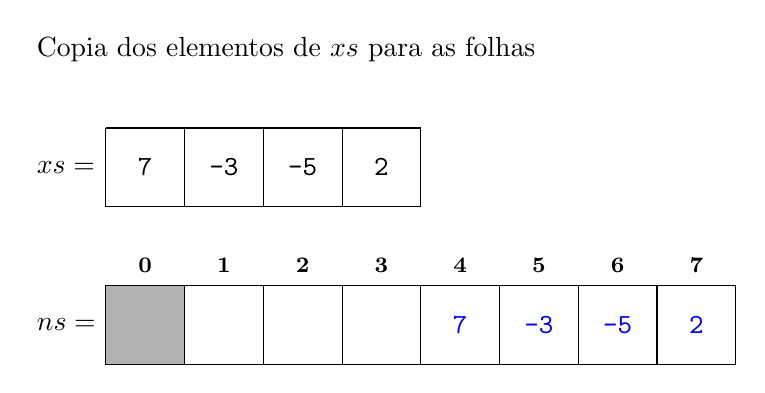
\begin{tikzpicture}
            \node[anchor=west] at (0, 5) { Copia dos elementos de $xs$ para as folhas };
            \node[anchor=west] at (0, 3.5) { $xs =$ };
            \node[anchor=west] at (0, 1.5) { $ns =$ };

            \draw[fill=gray!60] (1, 1) rectangle (2, 2);
            \draw (1, 3) grid (5, 4);
            \draw (1, 1) grid (9, 2);

            \node at (1.5, 2.25) { \footnotesize $\mathtt{\mathbf{0}}$ };
            \node at (2.5, 2.25) { \footnotesize $\mathtt{\mathbf{1}}$ };
            \node at (3.5, 2.25) { \footnotesize $\mathtt{\mathbf{2}}$ };
            \node at (4.5, 2.25) { \footnotesize $\mathtt{\mathbf{3}}$ };
            \node at (5.5, 2.25) { \footnotesize $\mathtt{\mathbf{4}}$ };
            \node at (6.5, 2.25) { \footnotesize $\mathtt{\mathbf{5}}$ };
            \node at (7.5, 2.25) { \footnotesize $\mathtt{\mathbf{6}}$ };
            \node at (8.5, 2.25) { \footnotesize $\mathtt{\mathbf{7}}$ };

            \node at (1.5, 3.5) { \tt 7 };
            \node at (2.5, 3.5) { \tt -3 };
            \node at (3.5, 3.5) { \tt -5 };
            \node at (4.5, 3.5) { \tt 2 };

            \node at (5.5, 1.5) { \tt \textcolor{blue}{7} };
            \node at (6.5, 1.5) { \tt \textcolor{blue}{-3} };
            \node at (7.5, 1.5) { \tt \textcolor{blue}{-5} };
            \node at (8.5, 1.5) { \tt \textcolor{blue}{2} };
        \end{tikzpicture}
    \end{figure}

\end{frame}

\begin{frame}[fragile]{Visualização do construtor da árvore de segmentos}

    \begin{figure}
        \centering

        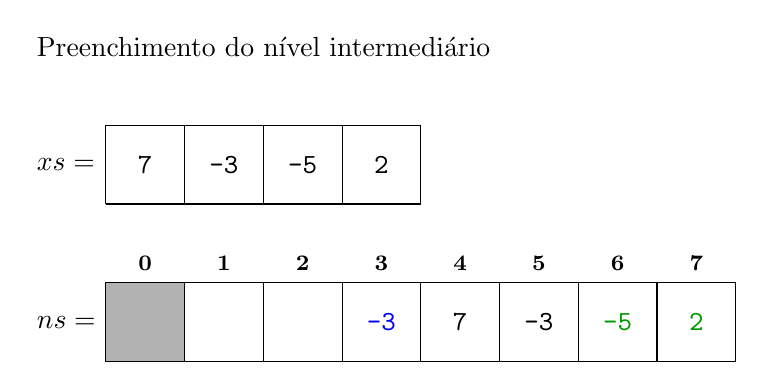
\begin{tikzpicture}
            \node[anchor=west] at (0, 5) { Preenchimento do nível intermediário };
            \node[anchor=west] at (0, 3.5) { $xs =$ };
            \node[anchor=west] at (0, 1.5) { $ns =$ };

            \draw[fill=gray!60] (1, 1) rectangle (2, 2);
            \draw (1, 3) grid (5, 4);
            \draw (1, 1) grid (9, 2);

            \node at (1.5, 2.25) { \footnotesize $\mathtt{\mathbf{0}}$ };
            \node at (2.5, 2.25) { \footnotesize $\mathtt{\mathbf{1}}$ };
            \node at (3.5, 2.25) { \footnotesize $\mathtt{\mathbf{2}}$ };
            \node at (4.5, 2.25) { \footnotesize $\mathtt{\mathbf{3}}$ };
            \node at (5.5, 2.25) { \footnotesize $\mathtt{\mathbf{4}}$ };
            \node at (6.5, 2.25) { \footnotesize $\mathtt{\mathbf{5}}$ };
            \node at (7.5, 2.25) { \footnotesize $\mathtt{\mathbf{6}}$ };
            \node at (8.5, 2.25) { \footnotesize $\mathtt{\mathbf{7}}$ };

            \node at (1.5, 3.5) { \tt 7 };
            \node at (2.5, 3.5) { \tt -3 };
            \node at (3.5, 3.5) { \tt -5 };
            \node at (4.5, 3.5) { \tt 2 };

            \node at (4.5, 1.5) { \tt \textcolor{blue}{-3} };
            \node at (5.5, 1.5) { \tt \textcolor{black}{7} };
            \node at (6.5, 1.5) { \tt \textcolor{black}{-3} };
            \node at (7.5, 1.5) { \tt \textcolor{green!60!black}{-5} };
            \node at (8.5, 1.5) { \tt \textcolor{green!60!black}{2} };
        \end{tikzpicture}
    \end{figure}

\end{frame}

\begin{frame}[fragile]{Visualização do construtor da árvore de segmentos}

    \begin{figure}
        \centering

        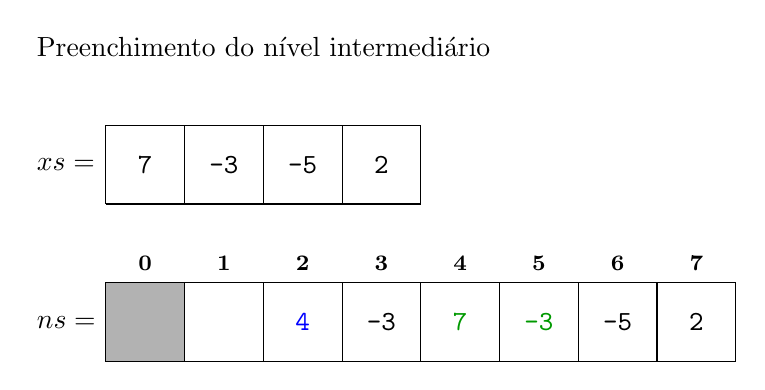
\begin{tikzpicture}
            \node[anchor=west] at (0, 5) { Preenchimento do nível intermediário };
            \node[anchor=west] at (0, 3.5) { $xs =$ };
            \node[anchor=west] at (0, 1.5) { $ns =$ };

            \draw[fill=gray!60] (1, 1) rectangle (2, 2);
            \draw (1, 3) grid (5, 4);
            \draw (1, 1) grid (9, 2);

            \node at (1.5, 2.25) { \footnotesize $\mathtt{\mathbf{0}}$ };
            \node at (2.5, 2.25) { \footnotesize $\mathtt{\mathbf{1}}$ };
            \node at (3.5, 2.25) { \footnotesize $\mathtt{\mathbf{2}}$ };
            \node at (4.5, 2.25) { \footnotesize $\mathtt{\mathbf{3}}$ };
            \node at (5.5, 2.25) { \footnotesize $\mathtt{\mathbf{4}}$ };
            \node at (6.5, 2.25) { \footnotesize $\mathtt{\mathbf{5}}$ };
            \node at (7.5, 2.25) { \footnotesize $\mathtt{\mathbf{6}}$ };
            \node at (8.5, 2.25) { \footnotesize $\mathtt{\mathbf{7}}$ };

            \node at (1.5, 3.5) { \tt 7 };
            \node at (2.5, 3.5) { \tt -3 };
            \node at (3.5, 3.5) { \tt -5 };
            \node at (4.5, 3.5) { \tt 2 };

            \node at (3.5, 1.5) { \tt \textcolor{blue}{4} };
            \node at (4.5, 1.5) { \tt \textcolor{black}{-3} };
            \node at (5.5, 1.5) { \tt \textcolor{green!60!black}{7} };
            \node at (6.5, 1.5) { \tt \textcolor{green!60!black}{-3} };
            \node at (7.5, 1.5) { \tt \textcolor{black}{-5} };
            \node at (8.5, 1.5) { \tt \textcolor{black}{2} };
        \end{tikzpicture}
    \end{figure}

\end{frame}

\begin{frame}[fragile]{Visualização do construtor da árvore de segmentos}

    \begin{figure}
        \centering

        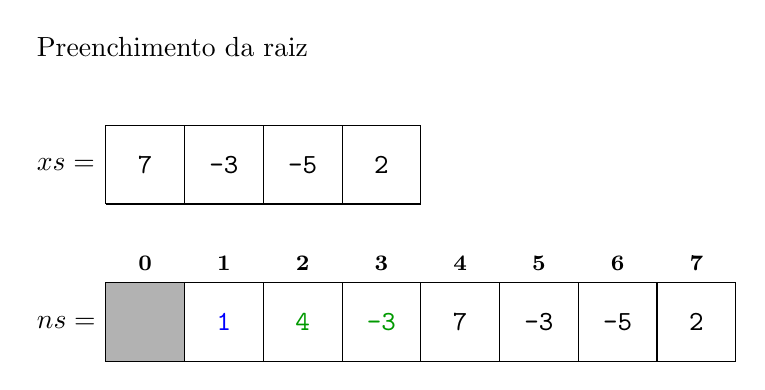
\begin{tikzpicture}
            \node[anchor=west] at (0, 5) { Preenchimento da raiz };
            \node[anchor=west] at (0, 3.5) { $xs =$ };
            \node[anchor=west] at (0, 1.5) { $ns =$ };

            \draw[fill=gray!60] (1, 1) rectangle (2, 2);
            \draw (1, 3) grid (5, 4);
            \draw (1, 1) grid (9, 2);

            \node at (1.5, 2.25) { \footnotesize $\mathtt{\mathbf{0}}$ };
            \node at (2.5, 2.25) { \footnotesize $\mathtt{\mathbf{1}}$ };
            \node at (3.5, 2.25) { \footnotesize $\mathtt{\mathbf{2}}$ };
            \node at (4.5, 2.25) { \footnotesize $\mathtt{\mathbf{3}}$ };
            \node at (5.5, 2.25) { \footnotesize $\mathtt{\mathbf{4}}$ };
            \node at (6.5, 2.25) { \footnotesize $\mathtt{\mathbf{5}}$ };
            \node at (7.5, 2.25) { \footnotesize $\mathtt{\mathbf{6}}$ };
            \node at (8.5, 2.25) { \footnotesize $\mathtt{\mathbf{7}}$ };

            \node at (1.5, 3.5) { \tt 7 };
            \node at (2.5, 3.5) { \tt -3 };
            \node at (3.5, 3.5) { \tt -5 };
            \node at (4.5, 3.5) { \tt 2 };

            \node at (2.5, 1.5) { \tt \textcolor{blue}{1} };
            \node at (3.5, 1.5) { \tt \textcolor{green!60!black}{4} };
            \node at (4.5, 1.5) { \tt \textcolor{green!60!black}{-3} };
            \node at (5.5, 1.5) { \tt \textcolor{black}{7} };
            \node at (6.5, 1.5) { \tt \textcolor{black}{-3} };
            \node at (7.5, 1.5) { \tt \textcolor{black}{-5} };
            \node at (8.5, 1.5) { \tt \textcolor{black}{2} };
        \end{tikzpicture}
    \end{figure}

\end{frame}


\begin{frame}[fragile]{Implementação do construtor da árvore de segmentos}
    \inputsnippet{cpp}{1}{21}{codes/segtree.h}
\end{frame}

\begin{frame}[fragile]{\it Range query}

    \begin{itemize}
        \item Uma vez inicializada a árvore de segmentos, é possível determinar o resultado
            da operação subjacente para um intervalo $[a, b]$ arbitrário

        \item Para isto, três observações devem ser feitas:
            \begin{enumerate}
                \item Se $a$ é ímpar, ele é o filho à direita, logo ele deve ser processado
                    separadamente

                \item O mesmo acontece se $b$ é par

                \item Nos outros casos, os valores de $a$ e $b$ já foram processados por seus
                    pais, e o processamento deve seguir para estes pais
            \end{enumerate}

        \item Assim, como a altura da árvore é igual a $\log N$, esta rotina tem complexidade
            $O(\log N)$

        \item Se a operação subjacente é a soma dos elementos, esta operação recebe o nome de
            \textit{range sum query} (RSQ)
    \end{itemize}

\end{frame}

\section{\it Range sum queries}

\begin{frame}[fragile]{\textit{Range sum query} em uma árvore de Fenwick}

    \begin{itemize}
        \item Considere que 
        \[
            [1, j] = I_{k_1} \cup I_{k_2} \cup \ldots I_{k_r},
        \]
        com $r = O(\log N)$, $I_a \cap I_b = \emptyset$ se $a\neq b$ e $I_k$ é o intervalo associado
        a $t_k$

        \item Por exemplo,
        \[
            [1, 15] = [1, 8]\cup [9, 12]\cup [13, 14]\cup [15, 15]
        \]

        \item Defina
        \[
            S(j) = \sum_{i = k_1}^{k_r} t_i
        \]

        \item Assim, fazendo $t_0 = 0$, segue que
        \[
            RSQ(i, j) = S(j) - S(i - 1)
        \]

    \end{itemize}

\end{frame}

\begin{frame}[fragile]{Identificação da decomposição de intervalos}

    \begin{itemize}
        \item Para encontrar a decomposição de um intervalo $[1, j]$ em intervalos disjuntos 
            associados aos elementos $t_k$, é preciso computar os valores de $p(n)$

        \item De fato, $p(n)$ corresponde ao \textit{bit} menos significativo de $n$ em base
            binária

        \item Este \textit{bit} pode ser determinado de forma eficiente através de uma operação
            binária
        \[
            p(n) = n \land (-n),
        \]
        onde $\land$ corresponde ao \lq\lq e\rq\rq\ lógico

        \item Os índices $r_i$ dos intervalos $I$ que decompõem $[1,j]$ formam a sequência
            de inteiros positivos 
        \[
            j, j - p(j), [j - p(j)] - p(j - p(j)), \ldots,
        \]
    \end{itemize}

\end{frame}

\begin{frame}[fragile]{Implementação da RSQ em uma BITree}
    \inputsnippet{cpp}{14}{33}{codes/ft.cpp}
\end{frame}

\begin{frame}[fragile]{Visualização de uma RSQ em uma BITree}

    \begin{figure}
        \centering

        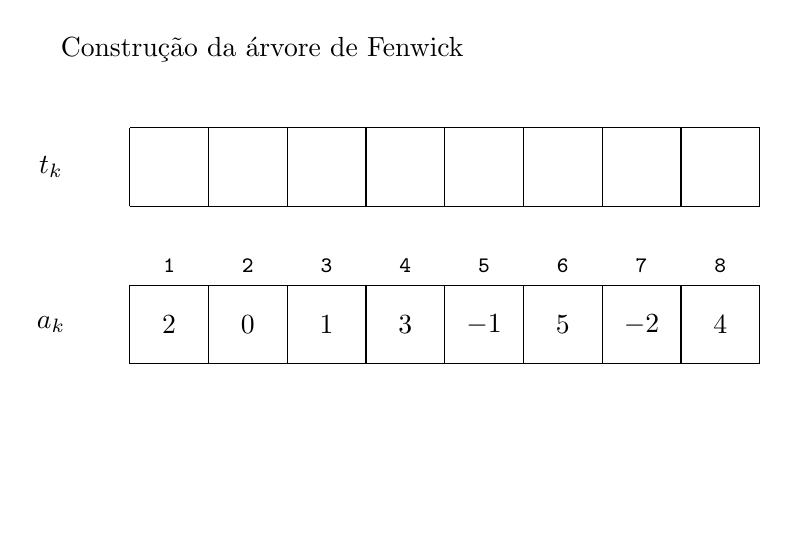
\begin{tikzpicture}
            \node[anchor=west] at (0, 12) { Construção da árvore de Fenwick };

            \draw (1, 10) grid (9, 11);
            \draw (1, 8) grid (9, 9);

            \node at (0, 8.5) { $a_k$ };
            \node at (0, 10.5) { $t_k$ };

            \node[opacity=0, anchor=west] at (0, 6.5) { $RSQ(3,7) = RSQ(1, 7) - RSQ(1, 2)$ };

            \node at (1.5, 9.25) { \footnotesize \tt 1 };
            \node at (2.5, 9.25) { \footnotesize \tt 2 };
            \node at (3.5, 9.25) { \footnotesize \tt 3 };
            \node at (4.5, 9.25) { \footnotesize \tt 4 };
            \node at (5.5, 9.25) { \footnotesize \tt 5 };
            \node at (6.5, 9.25) { \footnotesize \tt 6 };
            \node at (7.5, 9.25) { \footnotesize \tt 7 };
            \node at (8.5, 9.25) { \footnotesize \tt 8 };

            \node at (1.5, 8.5) { $2$ };
            \node at (2.5, 8.5) { $0$ };
            \node at (3.5, 8.5) { $1$ };
            \node at (4.5, 8.5) { $3$ };
            \node at (5.5, 8.5) { $-1$ };
            \node at (6.5, 8.5) { $5$ };
            \node at (7.5, 8.5) { $-2$ };
            \node at (8.5, 8.5) { $4$ };

        \end{tikzpicture}

    \end{figure}

\end{frame}

\begin{frame}[fragile]{Visualização de uma RSQ em uma BITree}

    \begin{figure}
        \centering

        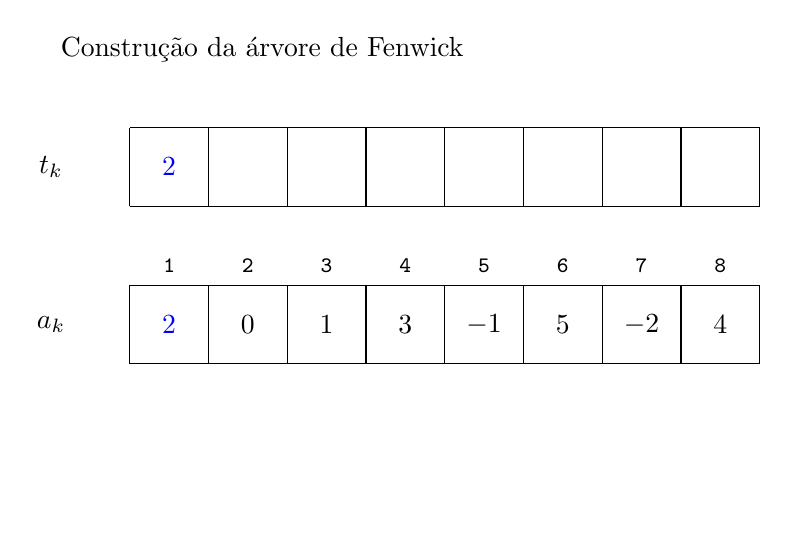
\begin{tikzpicture}
            \node[anchor=west] at (0, 12) { Construção da árvore de Fenwick };

            \draw (1, 10) grid (9, 11);
            \draw (1, 8) grid (9, 9);

            \node at (0, 8.5) { $a_k$ };
            \node at (0, 10.5) { $t_k$ };

            \node[opacity=0, anchor=west] at (0, 6.5) { $RSQ(3,7) = RSQ(1, 7) - RSQ(1, 2)$ };

            \node at (1.5, 9.25) { \footnotesize \tt 1 };
            \node at (2.5, 9.25) { \footnotesize \tt 2 };
            \node at (3.5, 9.25) { \footnotesize \tt 3 };
            \node at (4.5, 9.25) { \footnotesize \tt 4 };
            \node at (5.5, 9.25) { \footnotesize \tt 5 };
            \node at (6.5, 9.25) { \footnotesize \tt 6 };
            \node at (7.5, 9.25) { \footnotesize \tt 7 };
            \node at (8.5, 9.25) { \footnotesize \tt 8 };

            \node at (1.5, 8.5) { \textcolor{blue}{$2$} };
            \node at (2.5, 8.5) { $0$ };
            \node at (3.5, 8.5) { $1$ };
            \node at (4.5, 8.5) { $3$ };
            \node at (5.5, 8.5) { $-1$ };
            \node at (6.5, 8.5) { $5$ };
            \node at (7.5, 8.5) { $-2$ };
            \node at (8.5, 8.5) { $4$ };

            \node at (1.5, 10.5) { \textcolor{blue}{$2$} };
        \end{tikzpicture}

    \end{figure}

\end{frame}

\begin{frame}[fragile]{Visualização de uma RSQ em uma BITree}

    \begin{figure}
        \centering

        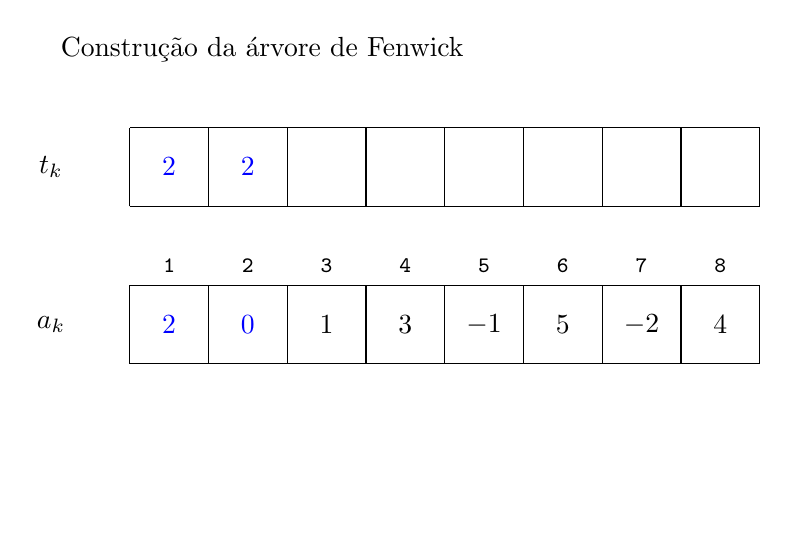
\begin{tikzpicture}
            \node[anchor=west] at (0, 12) { Construção da árvore de Fenwick };

            \draw (1, 10) grid (9, 11);
            \draw (1, 8) grid (9, 9);

            \node at (0, 8.5) { $a_k$ };
            \node at (0, 10.5) { $t_k$ };

            \node[opacity=0, anchor=west] at (0, 6.5) { $RSQ(3,7) = RSQ(1, 7) - RSQ(1, 2)$ };

            \node at (1.5, 9.25) { \footnotesize \tt 1 };
            \node at (2.5, 9.25) { \footnotesize \tt 2 };
            \node at (3.5, 9.25) { \footnotesize \tt 3 };
            \node at (4.5, 9.25) { \footnotesize \tt 4 };
            \node at (5.5, 9.25) { \footnotesize \tt 5 };
            \node at (6.5, 9.25) { \footnotesize \tt 6 };
            \node at (7.5, 9.25) { \footnotesize \tt 7 };
            \node at (8.5, 9.25) { \footnotesize \tt 8 };

            \node at (1.5, 8.5) { \textcolor{blue}{$2$} };
            \node at (2.5, 8.5) { \textcolor{blue}{$0$} };
            \node at (3.5, 8.5) { $1$ };
            \node at (4.5, 8.5) { $3$ };
            \node at (5.5, 8.5) { $-1$ };
            \node at (6.5, 8.5) { $5$ };
            \node at (7.5, 8.5) { $-2$ };
            \node at (8.5, 8.5) { $4$ };

            \node at (1.5, 10.5) { \textcolor{blue}{$2$} };
            \node at (2.5, 10.5) { \textcolor{blue}{$2$} };

        \end{tikzpicture}

    \end{figure}

\end{frame}

\begin{frame}[fragile]{Visualização de uma RSQ em uma BITree}

    \begin{figure}
        \centering

        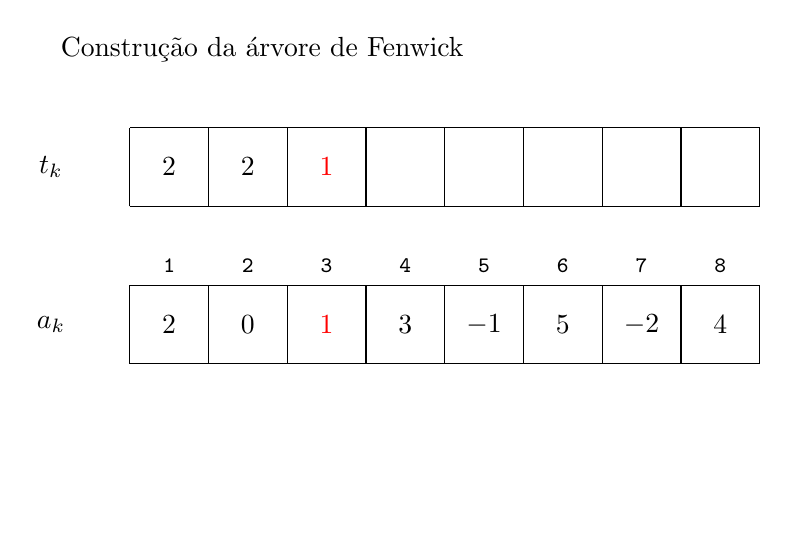
\begin{tikzpicture}
            \node[anchor=west] at (0, 12) { Construção da árvore de Fenwick };

            \draw (1, 10) grid (9, 11);
            \draw (1, 8) grid (9, 9);

            \node at (0, 8.5) { $a_k$ };
            \node at (0, 10.5) { $t_k$ };

            \node[opacity=0, anchor=west] at (0, 6.5) { $RSQ(3,7) = RSQ(1, 7) - RSQ(1, 2)$ };

            \node at (1.5, 9.25) { \footnotesize \tt 1 };
            \node at (2.5, 9.25) { \footnotesize \tt 2 };
            \node at (3.5, 9.25) { \footnotesize \tt 3 };
            \node at (4.5, 9.25) { \footnotesize \tt 4 };
            \node at (5.5, 9.25) { \footnotesize \tt 5 };
            \node at (6.5, 9.25) { \footnotesize \tt 6 };
            \node at (7.5, 9.25) { \footnotesize \tt 7 };
            \node at (8.5, 9.25) { \footnotesize \tt 8 };

            \node at (1.5, 8.5) { \textcolor{black}{$2$} };
            \node at (2.5, 8.5) { \textcolor{black}{$0$} };
            \node at (3.5, 8.5) { \textcolor{red}{$1$} };
            \node at (4.5, 8.5) { $3$ };
            \node at (5.5, 8.5) { $-1$ };
            \node at (6.5, 8.5) { $5$ };
            \node at (7.5, 8.5) { $-2$ };
            \node at (8.5, 8.5) { $4$ };

            \node at (1.5, 10.5) { \textcolor{black}{$2$} };
            \node at (2.5, 10.5) { \textcolor{black}{$2$} };
            \node at (3.5, 10.5) { \textcolor{red}{$1$} };

        \end{tikzpicture}

    \end{figure}

\end{frame}

\begin{frame}[fragile]{Visualização de uma RSQ em uma BITree}

    \begin{figure}
        \centering

        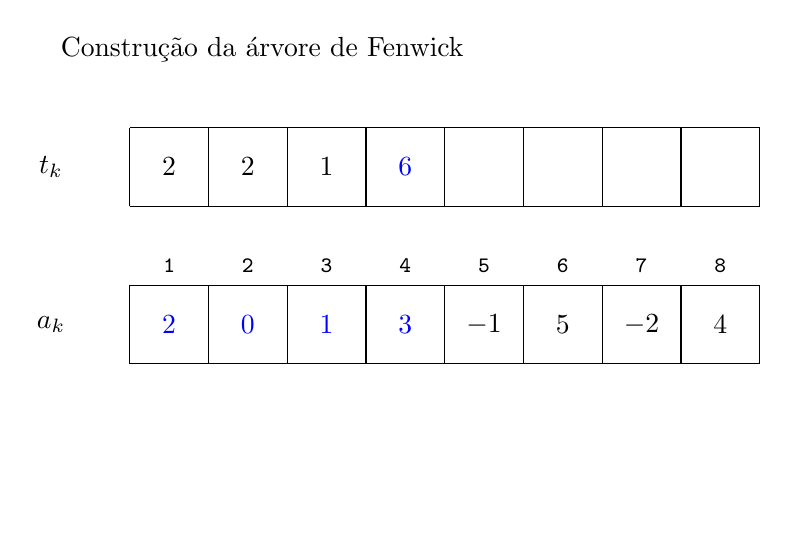
\begin{tikzpicture}
            \node[anchor=west] at (0, 12) { Construção da árvore de Fenwick };

            \draw (1, 10) grid (9, 11);
            \draw (1, 8) grid (9, 9);

            \node at (0, 8.5) { $a_k$ };
            \node at (0, 10.5) { $t_k$ };

            \node[opacity=0, anchor=west] at (0, 6.5) { $RSQ(3,7) = RSQ(1, 7) - RSQ(1, 2)$ };

            \node at (1.5, 9.25) { \footnotesize \tt 1 };
            \node at (2.5, 9.25) { \footnotesize \tt 2 };
            \node at (3.5, 9.25) { \footnotesize \tt 3 };
            \node at (4.5, 9.25) { \footnotesize \tt 4 };
            \node at (5.5, 9.25) { \footnotesize \tt 5 };
            \node at (6.5, 9.25) { \footnotesize \tt 6 };
            \node at (7.5, 9.25) { \footnotesize \tt 7 };
            \node at (8.5, 9.25) { \footnotesize \tt 8 };

            \node at (1.5, 8.5) { \textcolor{blue}{$2$} };
            \node at (2.5, 8.5) { \textcolor{blue}{$0$} };
            \node at (3.5, 8.5) { \textcolor{blue}{$1$} };
            \node at (4.5, 8.5) { \textcolor{blue}{$3$} };
            \node at (5.5, 8.5) { $-1$ };
            \node at (6.5, 8.5) { $5$ };
            \node at (7.5, 8.5) { $-2$ };
            \node at (8.5, 8.5) { $4$ };

            \node at (1.5, 10.5) { \textcolor{black}{$2$} };
            \node at (2.5, 10.5) { \textcolor{black}{$2$} };
            \node at (3.5, 10.5) { \textcolor{black}{$1$} };
            \node at (4.5, 10.5) { \textcolor{blue}{$6$} };

        \end{tikzpicture}

    \end{figure}

\end{frame}

\begin{frame}[fragile]{Visualização de uma RSQ em uma BITree}

    \begin{figure}
        \centering

        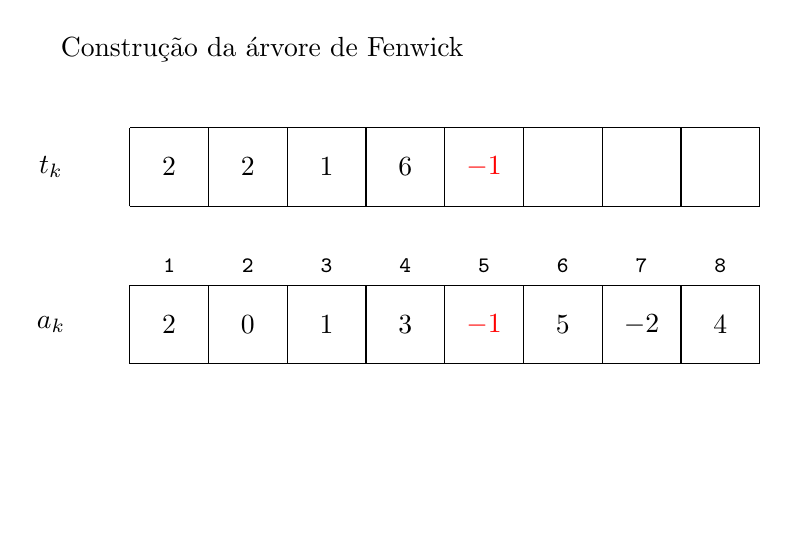
\begin{tikzpicture}
            \node[anchor=west] at (0, 12) { Construção da árvore de Fenwick };

            \draw (1, 10) grid (9, 11);
            \draw (1, 8) grid (9, 9);

            \node at (0, 8.5) { $a_k$ };
            \node at (0, 10.5) { $t_k$ };

            \node[opacity=0, anchor=west] at (0, 6.5) { $RSQ(3,7) = RSQ(1, 7) - RSQ(1, 2)$ };

            \node at (1.5, 9.25) { \footnotesize \tt 1 };
            \node at (2.5, 9.25) { \footnotesize \tt 2 };
            \node at (3.5, 9.25) { \footnotesize \tt 3 };
            \node at (4.5, 9.25) { \footnotesize \tt 4 };
            \node at (5.5, 9.25) { \footnotesize \tt 5 };
            \node at (6.5, 9.25) { \footnotesize \tt 6 };
            \node at (7.5, 9.25) { \footnotesize \tt 7 };
            \node at (8.5, 9.25) { \footnotesize \tt 8 };

            \node at (1.5, 8.5) { \textcolor{black}{$2$} };
            \node at (2.5, 8.5) { \textcolor{black}{$0$} };
            \node at (3.5, 8.5) { \textcolor{black}{$1$} };
            \node at (4.5, 8.5) { \textcolor{black}{$3$} };
            \node at (5.5, 8.5) { \textcolor{red}{$-1$} };
            \node at (6.5, 8.5) { $5$ };
            \node at (7.5, 8.5) { $-2$ };
            \node at (8.5, 8.5) { $4$ };

            \node at (1.5, 10.5) { \textcolor{black}{$2$} };
            \node at (2.5, 10.5) { \textcolor{black}{$2$} };
            \node at (3.5, 10.5) { \textcolor{black}{$1$} };
            \node at (4.5, 10.5) { \textcolor{black}{$6$} };
            \node at (5.5, 10.5) { \textcolor{red}{$-1$} };

        \end{tikzpicture}

    \end{figure}

\end{frame}

\begin{frame}[fragile]{Visualização de uma RSQ em uma BITree}

    \begin{figure}
        \centering

        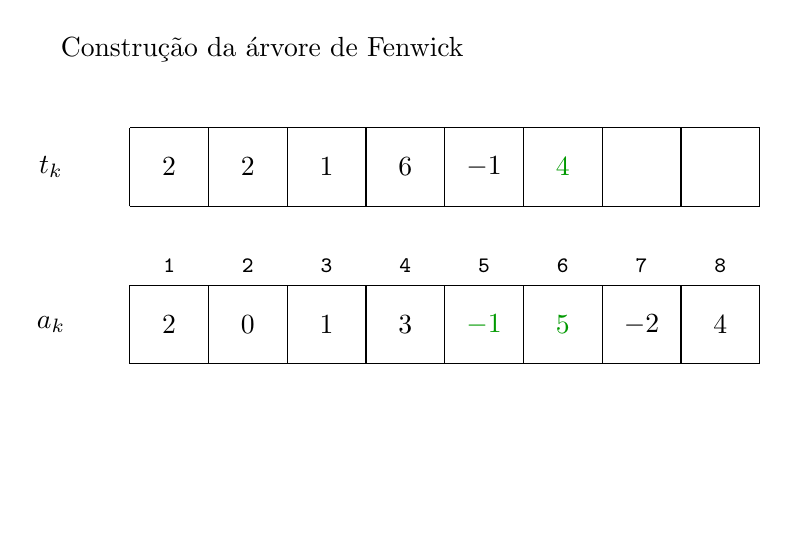
\begin{tikzpicture}
            \node[anchor=west] at (0, 12) { Construção da árvore de Fenwick };

            \draw (1, 10) grid (9, 11);
            \draw (1, 8) grid (9, 9);

            \node at (0, 8.5) { $a_k$ };
            \node at (0, 10.5) { $t_k$ };

            \node[opacity=0, anchor=west] at (0, 6.5) { $RSQ(3,7) = RSQ(1, 7) - RSQ(1, 2)$ };

            \node at (1.5, 9.25) { \footnotesize \tt 1 };
            \node at (2.5, 9.25) { \footnotesize \tt 2 };
            \node at (3.5, 9.25) { \footnotesize \tt 3 };
            \node at (4.5, 9.25) { \footnotesize \tt 4 };
            \node at (5.5, 9.25) { \footnotesize \tt 5 };
            \node at (6.5, 9.25) { \footnotesize \tt 6 };
            \node at (7.5, 9.25) { \footnotesize \tt 7 };
            \node at (8.5, 9.25) { \footnotesize \tt 8 };

            \node at (1.5, 8.5) { \textcolor{black}{$2$} };
            \node at (2.5, 8.5) { \textcolor{black}{$0$} };
            \node at (3.5, 8.5) { \textcolor{black}{$1$} };
            \node at (4.5, 8.5) { \textcolor{black}{$3$} };
            \node at (5.5, 8.5) { \textcolor{green!60!black}{$-1$} };
            \node at (6.5, 8.5) { \textcolor{green!60!black}{$5$} };
            \node at (7.5, 8.5) { $-2$ };
            \node at (8.5, 8.5) { $4$ };

            \node at (1.5, 10.5) { \textcolor{black}{$2$} };
            \node at (2.5, 10.5) { \textcolor{black}{$2$} };
            \node at (3.5, 10.5) { \textcolor{black}{$1$} };
            \node at (4.5, 10.5) { \textcolor{black}{$6$} };
            \node at (5.5, 10.5) { \textcolor{black}{$-1$} };
            \node at (6.5, 10.5) { \textcolor{green!60!black}{$4$} };

        \end{tikzpicture}

    \end{figure}

\end{frame}

\begin{frame}[fragile]{Visualização de uma RSQ em uma BITree}

    \begin{figure}
        \centering

        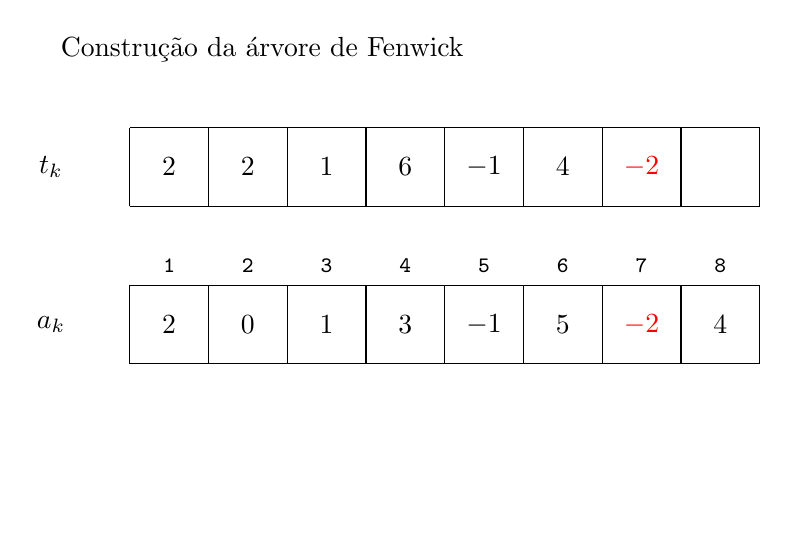
\begin{tikzpicture}
            \node[anchor=west] at (0, 12) { Construção da árvore de Fenwick };

            \draw (1, 10) grid (9, 11);
            \draw (1, 8) grid (9, 9);

            \node at (0, 8.5) { $a_k$ };
            \node at (0, 10.5) { $t_k$ };

            \node[opacity=0, anchor=west] at (0, 6.5) { $RSQ(3,7) = RSQ(1, 7) - RSQ(1, 2)$ };

            \node at (1.5, 9.25) { \footnotesize \tt 1 };
            \node at (2.5, 9.25) { \footnotesize \tt 2 };
            \node at (3.5, 9.25) { \footnotesize \tt 3 };
            \node at (4.5, 9.25) { \footnotesize \tt 4 };
            \node at (5.5, 9.25) { \footnotesize \tt 5 };
            \node at (6.5, 9.25) { \footnotesize \tt 6 };
            \node at (7.5, 9.25) { \footnotesize \tt 7 };
            \node at (8.5, 9.25) { \footnotesize \tt 8 };

            \node at (1.5, 8.5) { \textcolor{black}{$2$} };
            \node at (2.5, 8.5) { \textcolor{black}{$0$} };
            \node at (3.5, 8.5) { \textcolor{black}{$1$} };
            \node at (4.5, 8.5) { \textcolor{black}{$3$} };
            \node at (5.5, 8.5) { \textcolor{black}{$-1$} };
            \node at (6.5, 8.5) { \textcolor{black}{$5$} };
            \node at (7.5, 8.5) { \textcolor{red}{$-2$} };
            \node at (8.5, 8.5) { $4$ };

            \node at (1.5, 10.5) { \textcolor{black}{$2$} };
            \node at (2.5, 10.5) { \textcolor{black}{$2$} };
            \node at (3.5, 10.5) { \textcolor{black}{$1$} };
            \node at (4.5, 10.5) { \textcolor{black}{$6$} };
            \node at (5.5, 10.5) { \textcolor{black}{$-1$} };
            \node at (6.5, 10.5) { \textcolor{black}{$4$} };
            \node at (7.5, 10.5) { \textcolor{red}{$-2$} };

        \end{tikzpicture}

    \end{figure}

\end{frame}

\begin{frame}[fragile]{Visualização de uma RSQ em uma BITree}

    \begin{figure}
        \centering

        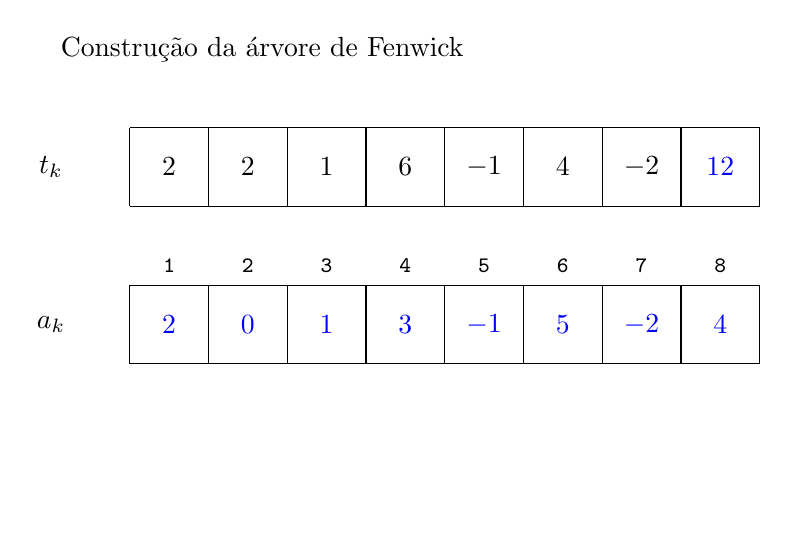
\begin{tikzpicture}
            \node[anchor=west] at (0, 12) { Construção da árvore de Fenwick };

            \draw (1, 10) grid (9, 11);
            \draw (1, 8) grid (9, 9);

            \node at (0, 8.5) { $a_k$ };
            \node at (0, 10.5) { $t_k$ };

            \node[opacity=0, anchor=west] at (0, 6.5) { $RSQ(3,7) = RSQ(1, 7) - RSQ(1, 2)$ };

            \node at (1.5, 9.25) { \footnotesize \tt 1 };
            \node at (2.5, 9.25) { \footnotesize \tt 2 };
            \node at (3.5, 9.25) { \footnotesize \tt 3 };
            \node at (4.5, 9.25) { \footnotesize \tt 4 };
            \node at (5.5, 9.25) { \footnotesize \tt 5 };
            \node at (6.5, 9.25) { \footnotesize \tt 6 };
            \node at (7.5, 9.25) { \footnotesize \tt 7 };
            \node at (8.5, 9.25) { \footnotesize \tt 8 };

            \node at (1.5, 8.5) { \textcolor{blue}{$2$} };
            \node at (2.5, 8.5) { \textcolor{blue}{$0$} };
            \node at (3.5, 8.5) { \textcolor{blue}{$1$} };
            \node at (4.5, 8.5) { \textcolor{blue}{$3$} };
            \node at (5.5, 8.5) { \textcolor{blue}{$-1$} };
            \node at (6.5, 8.5) { \textcolor{blue}{$5$} };
            \node at (7.5, 8.5) { \textcolor{blue}{$-2$} };
            \node at (8.5, 8.5) { \textcolor{blue}{$4$} };

            \node at (1.5, 10.5) { \textcolor{black}{$2$} };
            \node at (2.5, 10.5) { \textcolor{black}{$2$} };
            \node at (3.5, 10.5) { \textcolor{black}{$1$} };
            \node at (4.5, 10.5) { \textcolor{black}{$6$} };
            \node at (5.5, 10.5) { \textcolor{black}{$-1$} };
            \node at (6.5, 10.5) { \textcolor{black}{$4$} };
            \node at (7.5, 10.5) { \textcolor{black}{$-2$} };
            \node at (8.5, 10.5) { \textcolor{blue}{$12$} };

        \end{tikzpicture}

    \end{figure}

\end{frame}

\begin{frame}[fragile]{Visualização de uma RSQ em uma BITree}

    \begin{figure}
        \centering

        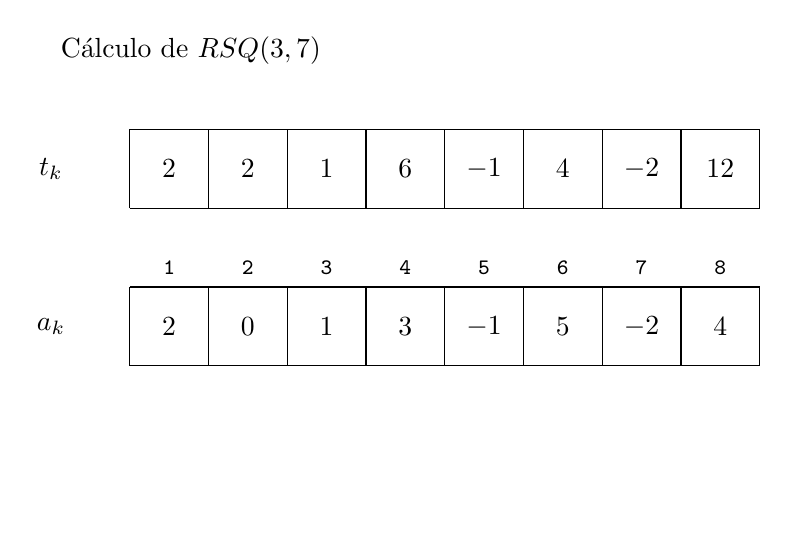
\begin{tikzpicture}
            \node[anchor=west] at (0, 12) { Cálculo de $RSQ(3, 7)$ };

            \draw (1, 10) grid (9, 11);
            \draw (1, 8) grid (9, 9);

            \node at (0, 8.5) { $a_k$ };
            \node at (0, 10.5) { $t_k$ };

            \node[opacity=0, anchor=west] at (0, 6.5) { $RSQ(3,7) = RSQ(1, 7) - RSQ(1, 2)$ };

            \node at (1.5, 9.25) { \footnotesize \tt 1 };
            \node at (2.5, 9.25) { \footnotesize \tt 2 };
            \node at (3.5, 9.25) { \footnotesize \tt 3 };
            \node at (4.5, 9.25) { \footnotesize \tt 4 };
            \node at (5.5, 9.25) { \footnotesize \tt 5 };
            \node at (6.5, 9.25) { \footnotesize \tt 6 };
            \node at (7.5, 9.25) { \footnotesize \tt 7 };
            \node at (8.5, 9.25) { \footnotesize \tt 8 };

            \node at (1.5, 8.5) { \textcolor{black}{$2$} };
            \node at (2.5, 8.5) { \textcolor{black}{$0$} };
            \node at (3.5, 8.5) { \textcolor{black}{$1$} };
            \node at (4.5, 8.5) { \textcolor{black}{$3$} };
            \node at (5.5, 8.5) { \textcolor{black}{$-1$} };
            \node at (6.5, 8.5) { \textcolor{black}{$5$} };
            \node at (7.5, 8.5) { \textcolor{black}{$-2$} };
            \node at (8.5, 8.5) { \textcolor{black}{$4$} };

            \node at (1.5, 10.5) { \textcolor{black}{$2$} };
            \node at (2.5, 10.5) { \textcolor{black}{$2$} };
            \node at (3.5, 10.5) { \textcolor{black}{$1$} };
            \node at (4.5, 10.5) { \textcolor{black}{$6$} };
            \node at (5.5, 10.5) { \textcolor{black}{$-1$} };
            \node at (6.5, 10.5) { \textcolor{black}{$4$} };
            \node at (7.5, 10.5) { \textcolor{black}{$-2$} };
            \node at (8.5, 10.5) { \textcolor{black}{$12$} };

        \end{tikzpicture}

    \end{figure}

\end{frame}

\begin{frame}[fragile]{Visualização de uma RSQ em uma BITree}

    \begin{figure}
        \centering

        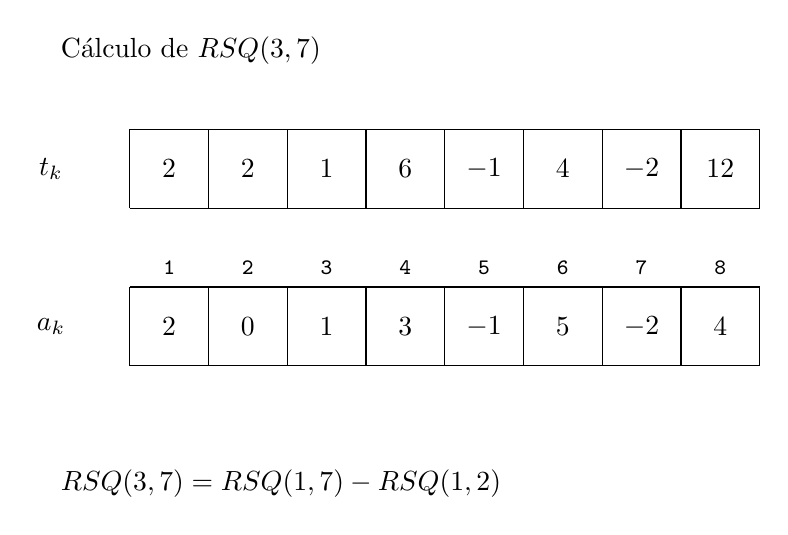
\begin{tikzpicture}
            \node[anchor=west] at (0, 12) { Cálculo de $RSQ(3, 7)$ };

            \draw (1, 10) grid (9, 11);
            \draw (1, 8) grid (9, 9);

            \node at (0, 8.5) { $a_k$ };
            \node at (0, 10.5) { $t_k$ };

            \node[anchor=west] at (0, 6.5) { $RSQ(3,7) = RSQ(1, 7) - RSQ(1, 2)$ };

            \node at (1.5, 9.25) { \footnotesize \tt 1 };
            \node at (2.5, 9.25) { \footnotesize \tt 2 };
            \node at (3.5, 9.25) { \footnotesize \tt 3 };
            \node at (4.5, 9.25) { \footnotesize \tt 4 };
            \node at (5.5, 9.25) { \footnotesize \tt 5 };
            \node at (6.5, 9.25) { \footnotesize \tt 6 };
            \node at (7.5, 9.25) { \footnotesize \tt 7 };
            \node at (8.5, 9.25) { \footnotesize \tt 8 };

            \node at (1.5, 8.5) { \textcolor{black}{$2$} };
            \node at (2.5, 8.5) { \textcolor{black}{$0$} };
            \node at (3.5, 8.5) { \textcolor{black}{$1$} };
            \node at (4.5, 8.5) { \textcolor{black}{$3$} };
            \node at (5.5, 8.5) { \textcolor{black}{$-1$} };
            \node at (6.5, 8.5) { \textcolor{black}{$5$} };
            \node at (7.5, 8.5) { \textcolor{black}{$-2$} };
            \node at (8.5, 8.5) { \textcolor{black}{$4$} };

            \node at (1.5, 10.5) { \textcolor{black}{$2$} };
            \node at (2.5, 10.5) { \textcolor{black}{$2$} };
            \node at (3.5, 10.5) { \textcolor{black}{$1$} };
            \node at (4.5, 10.5) { \textcolor{black}{$6$} };
            \node at (5.5, 10.5) { \textcolor{black}{$-1$} };
            \node at (6.5, 10.5) { \textcolor{black}{$4$} };
            \node at (7.5, 10.5) { \textcolor{black}{$-2$} };
            \node at (8.5, 10.5) { \textcolor{black}{$12$} };

        \end{tikzpicture}

    \end{figure}

\end{frame}

\begin{frame}[fragile]{Visualização de uma RSQ em uma BITree}

    \begin{figure}
        \centering

        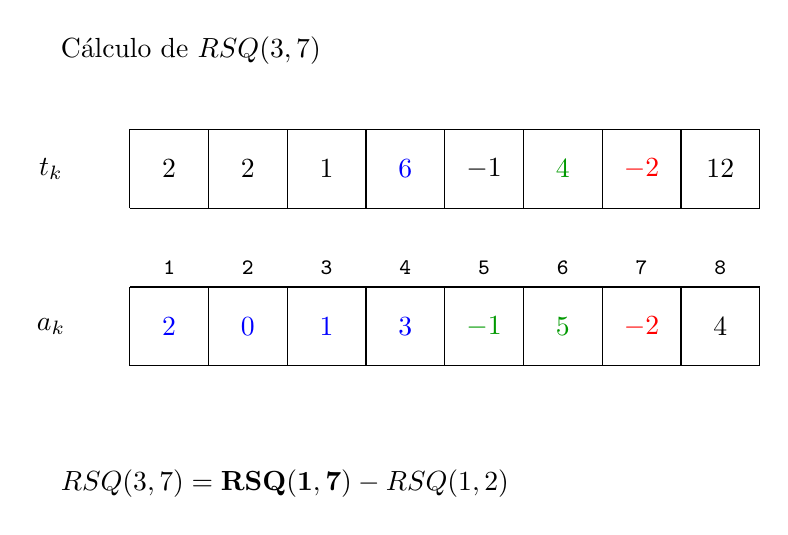
\begin{tikzpicture}
            \node[anchor=west] at (0, 12) { Cálculo de $RSQ(3, 7)$ };

            \draw (1, 10) grid (9, 11);
            \draw (1, 8) grid (9, 9);

            \node at (0, 8.5) { $a_k$ };
            \node at (0, 10.5) { $t_k$ };

            \node[anchor=west] at (0, 6.5) { $RSQ(3,7) = \mathbf{RSQ(1, 7)} - RSQ(1, 2)$ };

            \node at (1.5, 9.25) { \footnotesize \tt 1 };
            \node at (2.5, 9.25) { \footnotesize \tt 2 };
            \node at (3.5, 9.25) { \footnotesize \tt 3 };
            \node at (4.5, 9.25) { \footnotesize \tt 4 };
            \node at (5.5, 9.25) { \footnotesize \tt 5 };
            \node at (6.5, 9.25) { \footnotesize \tt 6 };
            \node at (7.5, 9.25) { \footnotesize \tt 7 };
            \node at (8.5, 9.25) { \footnotesize \tt 8 };

            \node at (1.5, 8.5) { \textcolor{blue}{$2$} };
            \node at (2.5, 8.5) { \textcolor{blue}{$0$} };
            \node at (3.5, 8.5) { \textcolor{blue}{$1$} };
            \node at (4.5, 8.5) { \textcolor{blue}{$3$} };
            \node at (5.5, 8.5) { \textcolor{green!60!black}{$-1$} };
            \node at (6.5, 8.5) { \textcolor{green!60!black}{$5$} };
            \node at (7.5, 8.5) { \textcolor{red}{$-2$} };
            \node at (8.5, 8.5) { \textcolor{black}{$4$} };

            \node at (1.5, 10.5) { \textcolor{black}{$2$} };
            \node at (2.5, 10.5) { \textcolor{black}{$2$} };
            \node at (3.5, 10.5) { \textcolor{black}{$1$} };
            \node at (4.5, 10.5) { \textcolor{blue}{$6$} };
            \node at (5.5, 10.5) { \textcolor{black}{$-1$} };
            \node at (6.5, 10.5) { \textcolor{green!60!black}{$4$} };
            \node at (7.5, 10.5) { \textcolor{red}{$-2$} };
            \node at (8.5, 10.5) { \textcolor{black}{$12$} };

        \end{tikzpicture}

    \end{figure}

\end{frame}

\begin{frame}[fragile]{Visualização de uma RSQ em uma BITree}

    \begin{figure}
        \centering

        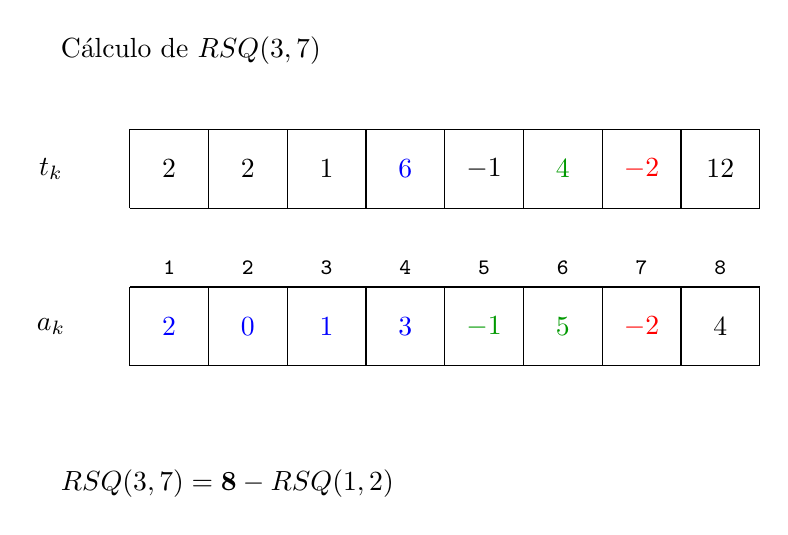
\begin{tikzpicture}
            \node[anchor=west] at (0, 12) { Cálculo de $RSQ(3, 7)$ };

            \draw (1, 10) grid (9, 11);
            \draw (1, 8) grid (9, 9);

            \node at (0, 8.5) { $a_k$ };
            \node at (0, 10.5) { $t_k$ };

            \node[anchor=west] at (0, 6.5) { $RSQ(3,7) = \mathbf{8} - RSQ(1, 2)$ };

            \node at (1.5, 9.25) { \footnotesize \tt 1 };
            \node at (2.5, 9.25) { \footnotesize \tt 2 };
            \node at (3.5, 9.25) { \footnotesize \tt 3 };
            \node at (4.5, 9.25) { \footnotesize \tt 4 };
            \node at (5.5, 9.25) { \footnotesize \tt 5 };
            \node at (6.5, 9.25) { \footnotesize \tt 6 };
            \node at (7.5, 9.25) { \footnotesize \tt 7 };
            \node at (8.5, 9.25) { \footnotesize \tt 8 };

            \node at (1.5, 8.5) { \textcolor{blue}{$2$} };
            \node at (2.5, 8.5) { \textcolor{blue}{$0$} };
            \node at (3.5, 8.5) { \textcolor{blue}{$1$} };
            \node at (4.5, 8.5) { \textcolor{blue}{$3$} };
            \node at (5.5, 8.5) { \textcolor{green!60!black}{$-1$} };
            \node at (6.5, 8.5) { \textcolor{green!60!black}{$5$} };
            \node at (7.5, 8.5) { \textcolor{red}{$-2$} };
            \node at (8.5, 8.5) { \textcolor{black}{$4$} };

            \node at (1.5, 10.5) { \textcolor{black}{$2$} };
            \node at (2.5, 10.5) { \textcolor{black}{$2$} };
            \node at (3.5, 10.5) { \textcolor{black}{$1$} };
            \node at (4.5, 10.5) { \textcolor{blue}{$6$} };
            \node at (5.5, 10.5) { \textcolor{black}{$-1$} };
            \node at (6.5, 10.5) { \textcolor{green!60!black}{$4$} };
            \node at (7.5, 10.5) { \textcolor{red}{$-2$} };
            \node at (8.5, 10.5) { \textcolor{black}{$12$} };

        \end{tikzpicture}

    \end{figure}

\end{frame}

\begin{frame}[fragile]{Visualização de uma RSQ em uma BITree}

    \begin{figure}
        \centering

        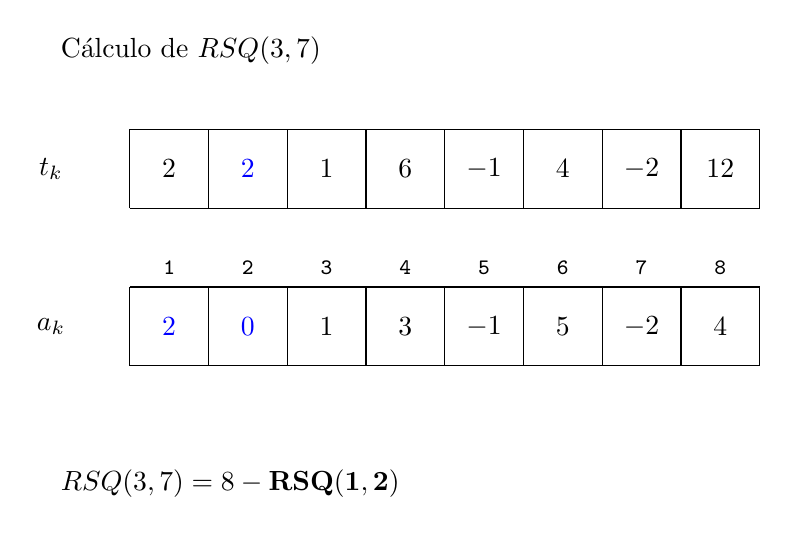
\begin{tikzpicture}
            \node[anchor=west] at (0, 12) { Cálculo de $RSQ(3, 7)$ };

            \draw (1, 10) grid (9, 11);
            \draw (1, 8) grid (9, 9);

            \node at (0, 8.5) { $a_k$ };
            \node at (0, 10.5) { $t_k$ };

            \node[anchor=west] at (0, 6.5) { $RSQ(3,7) = 8 - \mathbf{RSQ(1, 2)}$ };

            \node at (1.5, 9.25) { \footnotesize \tt 1 };
            \node at (2.5, 9.25) { \footnotesize \tt 2 };
            \node at (3.5, 9.25) { \footnotesize \tt 3 };
            \node at (4.5, 9.25) { \footnotesize \tt 4 };
            \node at (5.5, 9.25) { \footnotesize \tt 5 };
            \node at (6.5, 9.25) { \footnotesize \tt 6 };
            \node at (7.5, 9.25) { \footnotesize \tt 7 };
            \node at (8.5, 9.25) { \footnotesize \tt 8 };

            \node at (1.5, 8.5) { \textcolor{blue}{$2$} };
            \node at (2.5, 8.5) { \textcolor{blue}{$0$} };
            \node at (3.5, 8.5) { \textcolor{black}{$1$} };
            \node at (4.5, 8.5) { \textcolor{black}{$3$} };
            \node at (5.5, 8.5) { \textcolor{black}{$-1$} };
            \node at (6.5, 8.5) { \textcolor{black}{$5$} };
            \node at (7.5, 8.5) { \textcolor{black}{$-2$} };
            \node at (8.5, 8.5) { \textcolor{black}{$4$} };

            \node at (1.5, 10.5) { \textcolor{black}{$2$} };
            \node at (2.5, 10.5) { \textcolor{blue}{$2$} };
            \node at (3.5, 10.5) { \textcolor{black}{$1$} };
            \node at (4.5, 10.5) { \textcolor{black}{$6$} };
            \node at (5.5, 10.5) { \textcolor{black}{$-1$} };
            \node at (6.5, 10.5) { \textcolor{black}{$4$} };
            \node at (7.5, 10.5) { \textcolor{black}{$-2$} };
            \node at (8.5, 10.5) { \textcolor{black}{$12$} };

        \end{tikzpicture}

    \end{figure}

\end{frame}

\begin{frame}[fragile]{Visualização de uma RSQ em uma BITree}

    \begin{figure}
        \centering

        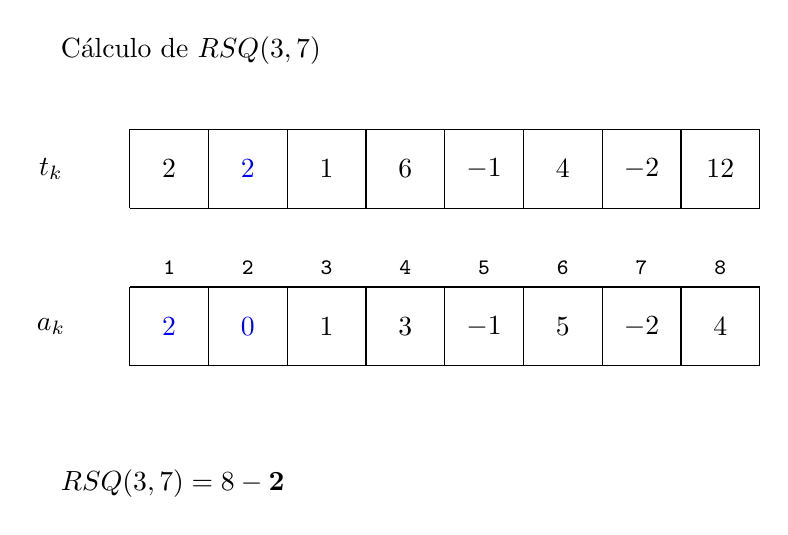
\begin{tikzpicture}
            \node[anchor=west] at (0, 12) { Cálculo de $RSQ(3, 7)$ };

            \draw (1, 10) grid (9, 11);
            \draw (1, 8) grid (9, 9);

            \node at (0, 8.5) { $a_k$ };
            \node at (0, 10.5) { $t_k$ };

            \node[anchor=west] at (0, 6.5) { $RSQ(3,7) = 8 - \mathbf{2}$ };

            \node at (1.5, 9.25) { \footnotesize \tt 1 };
            \node at (2.5, 9.25) { \footnotesize \tt 2 };
            \node at (3.5, 9.25) { \footnotesize \tt 3 };
            \node at (4.5, 9.25) { \footnotesize \tt 4 };
            \node at (5.5, 9.25) { \footnotesize \tt 5 };
            \node at (6.5, 9.25) { \footnotesize \tt 6 };
            \node at (7.5, 9.25) { \footnotesize \tt 7 };
            \node at (8.5, 9.25) { \footnotesize \tt 8 };

            \node at (1.5, 8.5) { \textcolor{blue}{$2$} };
            \node at (2.5, 8.5) { \textcolor{blue}{$0$} };
            \node at (3.5, 8.5) { \textcolor{black}{$1$} };
            \node at (4.5, 8.5) { \textcolor{black}{$3$} };
            \node at (5.5, 8.5) { \textcolor{black}{$-1$} };
            \node at (6.5, 8.5) { \textcolor{black}{$5$} };
            \node at (7.5, 8.5) { \textcolor{black}{$-2$} };
            \node at (8.5, 8.5) { \textcolor{black}{$4$} };

            \node at (1.5, 10.5) { \textcolor{black}{$2$} };
            \node at (2.5, 10.5) { \textcolor{blue}{$2$} };
            \node at (3.5, 10.5) { \textcolor{black}{$1$} };
            \node at (4.5, 10.5) { \textcolor{black}{$6$} };
            \node at (5.5, 10.5) { \textcolor{black}{$-1$} };
            \node at (6.5, 10.5) { \textcolor{black}{$4$} };
            \node at (7.5, 10.5) { \textcolor{black}{$-2$} };
            \node at (8.5, 10.5) { \textcolor{black}{$12$} };

        \end{tikzpicture}

    \end{figure}

\end{frame}

\begin{frame}[fragile]{Visualização de uma RSQ em uma BITree}

    \begin{figure}
        \centering

        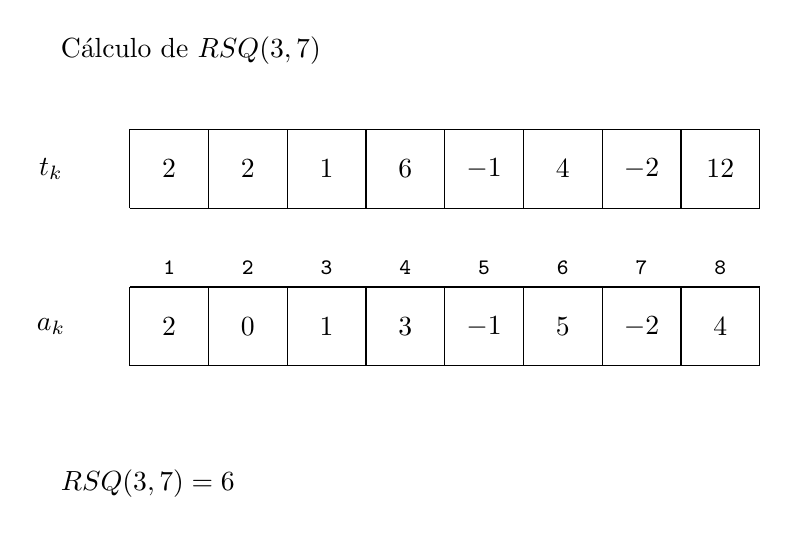
\begin{tikzpicture}
            \node[anchor=west] at (0, 12) { Cálculo de $RSQ(3, 7)$ };

            \draw (1, 10) grid (9, 11);
            \draw (1, 8) grid (9, 9);

            \node at (0, 8.5) { $a_k$ };
            \node at (0, 10.5) { $t_k$ };

            \node[anchor=west] at (0, 6.5) { $RSQ(3,7) = 6 $ };

            \node at (1.5, 9.25) { \footnotesize \tt 1 };
            \node at (2.5, 9.25) { \footnotesize \tt 2 };
            \node at (3.5, 9.25) { \footnotesize \tt 3 };
            \node at (4.5, 9.25) { \footnotesize \tt 4 };
            \node at (5.5, 9.25) { \footnotesize \tt 5 };
            \node at (6.5, 9.25) { \footnotesize \tt 6 };
            \node at (7.5, 9.25) { \footnotesize \tt 7 };
            \node at (8.5, 9.25) { \footnotesize \tt 8 };

            \node at (1.5, 8.5) { \textcolor{black}{$2$} };
            \node at (2.5, 8.5) { \textcolor{black}{$0$} };
            \node at (3.5, 8.5) { \textcolor{black}{$1$} };
            \node at (4.5, 8.5) { \textcolor{black}{$3$} };
            \node at (5.5, 8.5) { \textcolor{black}{$-1$} };
            \node at (6.5, 8.5) { \textcolor{black}{$5$} };
            \node at (7.5, 8.5) { \textcolor{black}{$-2$} };
            \node at (8.5, 8.5) { \textcolor{black}{$4$} };

            \node at (1.5, 10.5) { \textcolor{black}{$2$} };
            \node at (2.5, 10.5) { \textcolor{black}{$2$} };
            \node at (3.5, 10.5) { \textcolor{black}{$1$} };
            \node at (4.5, 10.5) { \textcolor{black}{$6$} };
            \node at (5.5, 10.5) { \textcolor{black}{$-1$} };
            \node at (6.5, 10.5) { \textcolor{black}{$4$} };
            \node at (7.5, 10.5) { \textcolor{black}{$-2$} };
            \node at (8.5, 10.5) { \textcolor{black}{$12$} };

        \end{tikzpicture}

    \end{figure}

\end{frame}


\begin{frame}[fragile]{Implementação da {\it range query}}
    \inputsnippet{cpp}{22}{42}{codes/segtree.h}
\end{frame}

\begin{frame}[fragile]{\it Update}

    \begin{itemize}
        \item A operação de atualização (\texttt{update(i, value)}) permite modificar o valor do
            elemento $ns[i]$

        \item O procedimento padrão é aplicar a operação subjacente ao atual valor de $ns[i]$
            e um parâmetro \texttt{value}

        \item Uma variante comum é a substituição do valor

        \item Neste caso, é preciso determinar qual seria o valor atual $x$ e então aplicar a
            atualização com o parâmetro \texttt{value} igual ao inverso de $x$ em relação à
            operação subjacente

        \item Uma vez modificado o valor, é preciso ir atualizado todos seus antepassados na
            árvore: pai, avô, etc, até a raiz

        \item Como a altura da árvore é igual a $\log N$, esta operação também tem complexidade
            $O(\log N)$
    \end{itemize}

\end{frame}

\begin{frame}[fragile]{Visualização de uma atualização em uma BITree}

    \begin{figure}
        \centering

        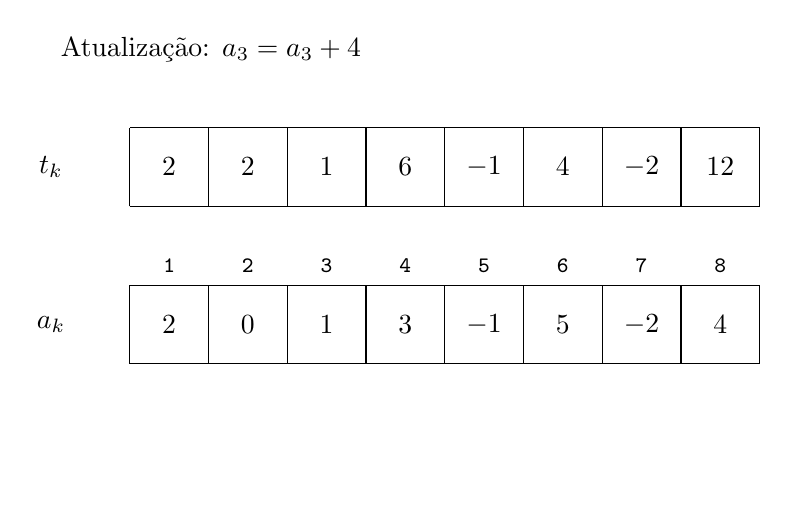
\begin{tikzpicture}
            \node[anchor=west] at (0, 12) { Atualização: $a_3 = a_3 + 4$ };

            \draw (1, 10) grid (9, 11);
            \draw (1, 8) grid (9, 9);

            \node at (0, 8.5) { $a_k$ };
            \node at (0, 10.5) { $t_k$ };

            \node[opacity=0, anchor=west] at (0, 6.5) { $r_1 = 3$ };

            \node at (1.5, 9.25) { \footnotesize \tt 1 };
            \node at (2.5, 9.25) { \footnotesize \tt 2 };
            \node at (3.5, 9.25) { \footnotesize \tt 3 };
            \node at (4.5, 9.25) { \footnotesize \tt 4 };
            \node at (5.5, 9.25) { \footnotesize \tt 5 };
            \node at (6.5, 9.25) { \footnotesize \tt 6 };
            \node at (7.5, 9.25) { \footnotesize \tt 7 };
            \node at (8.5, 9.25) { \footnotesize \tt 8 };

            \node at (1.5, 8.5) { \textcolor{black}{$2$} };
            \node at (2.5, 8.5) { \textcolor{black}{$0$} };
            \node at (3.5, 8.5) { \textcolor{black}{$1$} };
            \node at (4.5, 8.5) { \textcolor{black}{$3$} };
            \node at (5.5, 8.5) { \textcolor{black}{$-1$} };
            \node at (6.5, 8.5) { \textcolor{black}{$5$} };
            \node at (7.5, 8.5) { \textcolor{black}{$-2$} };
            \node at (8.5, 8.5) { \textcolor{black}{$4$} };

            \node at (1.5, 10.5) { \textcolor{black}{$2$} };
            \node at (2.5, 10.5) { \textcolor{black}{$2$} };
            \node at (3.5, 10.5) { \textcolor{black}{$1$} };
            \node at (4.5, 10.5) { \textcolor{black}{$6$} };
            \node at (5.5, 10.5) { \textcolor{black}{$-1$} };
            \node at (6.5, 10.5) { \textcolor{black}{$4$} };
            \node at (7.5, 10.5) { \textcolor{black}{$-2$} };
            \node at (8.5, 10.5) { \textcolor{black}{$12$} };

        \end{tikzpicture}

    \end{figure}

\end{frame}

\begin{frame}[fragile]{Visualização de uma atualização em uma BITree}

    \begin{figure}
        \centering

        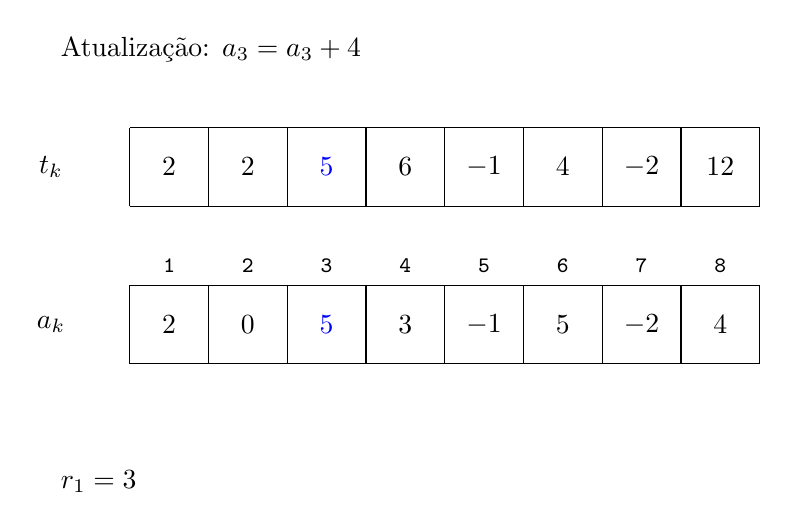
\begin{tikzpicture}
            \node[anchor=west] at (0, 12) { Atualização: $a_3 = a_3 + 4$ };

            \draw (1, 10) grid (9, 11);
            \draw (1, 8) grid (9, 9);

            \node at (0, 8.5) { $a_k$ };
            \node at (0, 10.5) { $t_k$ };

            \node[anchor=west] at (0, 6.5) { $r_1 = 3$ };

            \node at (1.5, 9.25) { \footnotesize \tt 1 };
            \node at (2.5, 9.25) { \footnotesize \tt 2 };
            \node at (3.5, 9.25) { \footnotesize \tt 3 };
            \node at (4.5, 9.25) { \footnotesize \tt 4 };
            \node at (5.5, 9.25) { \footnotesize \tt 5 };
            \node at (6.5, 9.25) { \footnotesize \tt 6 };
            \node at (7.5, 9.25) { \footnotesize \tt 7 };
            \node at (8.5, 9.25) { \footnotesize \tt 8 };

            \node at (1.5, 8.5) { \textcolor{black}{$2$} };
            \node at (2.5, 8.5) { \textcolor{black}{$0$} };
            \node at (3.5, 8.5) { \textcolor{blue}{$5$} };
            \node at (4.5, 8.5) { \textcolor{black}{$3$} };
            \node at (5.5, 8.5) { \textcolor{black}{$-1$} };
            \node at (6.5, 8.5) { \textcolor{black}{$5$} };
            \node at (7.5, 8.5) { \textcolor{black}{$-2$} };
            \node at (8.5, 8.5) { \textcolor{black}{$4$} };

            \node at (1.5, 10.5) { \textcolor{black}{$2$} };
            \node at (2.5, 10.5) { \textcolor{black}{$2$} };
            \node at (3.5, 10.5) { \textcolor{blue}{$5$} };
            \node at (4.5, 10.5) { \textcolor{black}{$6$} };
            \node at (5.5, 10.5) { \textcolor{black}{$-1$} };
            \node at (6.5, 10.5) { \textcolor{black}{$4$} };
            \node at (7.5, 10.5) { \textcolor{black}{$-2$} };
            \node at (8.5, 10.5) { \textcolor{black}{$12$} };

        \end{tikzpicture}

    \end{figure}

\end{frame}

\begin{frame}[fragile]{Visualização de uma atualização em uma BITree}

    \begin{figure}
        \centering

        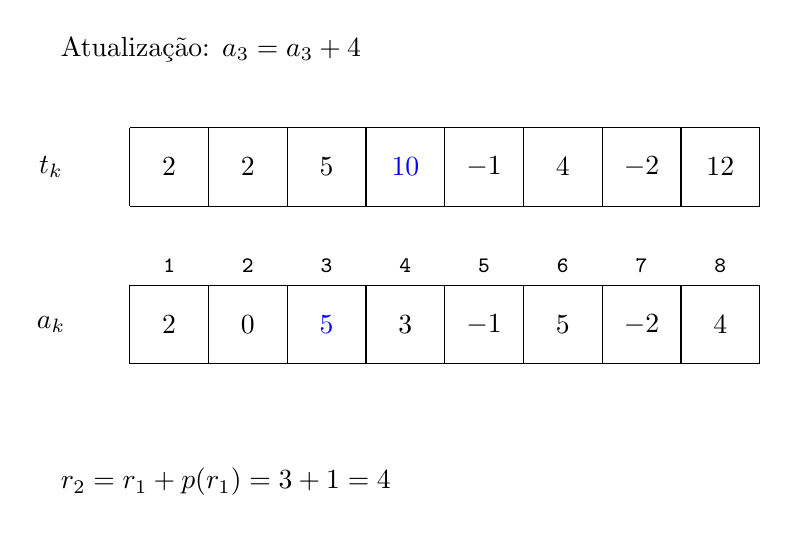
\begin{tikzpicture}
            \node[anchor=west] at (0, 12) { Atualização: $a_3 = a_3 + 4$ };

            \draw (1, 10) grid (9, 11);
            \draw (1, 8) grid (9, 9);

            \node at (0, 8.5) { $a_k$ };
            \node at (0, 10.5) { $t_k$ };

            \node[anchor=west] at (0, 6.5) { $r_2 = r_1 + p(r_1) = 3 + 1 = 4$ };

            \node at (1.5, 9.25) { \footnotesize \tt 1 };
            \node at (2.5, 9.25) { \footnotesize \tt 2 };
            \node at (3.5, 9.25) { \footnotesize \tt 3 };
            \node at (4.5, 9.25) { \footnotesize \tt 4 };
            \node at (5.5, 9.25) { \footnotesize \tt 5 };
            \node at (6.5, 9.25) { \footnotesize \tt 6 };
            \node at (7.5, 9.25) { \footnotesize \tt 7 };
            \node at (8.5, 9.25) { \footnotesize \tt 8 };

            \node at (1.5, 8.5) { \textcolor{black}{$2$} };
            \node at (2.5, 8.5) { \textcolor{black}{$0$} };
            \node at (3.5, 8.5) { \textcolor{blue}{$5$} };
            \node at (4.5, 8.5) { \textcolor{black}{$3$} };
            \node at (5.5, 8.5) { \textcolor{black}{$-1$} };
            \node at (6.5, 8.5) { \textcolor{black}{$5$} };
            \node at (7.5, 8.5) { \textcolor{black}{$-2$} };
            \node at (8.5, 8.5) { \textcolor{black}{$4$} };

            \node at (1.5, 10.5) { \textcolor{black}{$2$} };
            \node at (2.5, 10.5) { \textcolor{black}{$2$} };
            \node at (3.5, 10.5) { \textcolor{black}{$5$} };
            \node at (4.5, 10.5) { \textcolor{blue}{$10$} };
            \node at (5.5, 10.5) { \textcolor{black}{$-1$} };
            \node at (6.5, 10.5) { \textcolor{black}{$4$} };
            \node at (7.5, 10.5) { \textcolor{black}{$-2$} };
            \node at (8.5, 10.5) { \textcolor{black}{$12$} };

        \end{tikzpicture}

    \end{figure}

\end{frame}

\begin{frame}[fragile]{Visualização de uma atualização em uma BITree}

    \begin{figure}
        \centering

        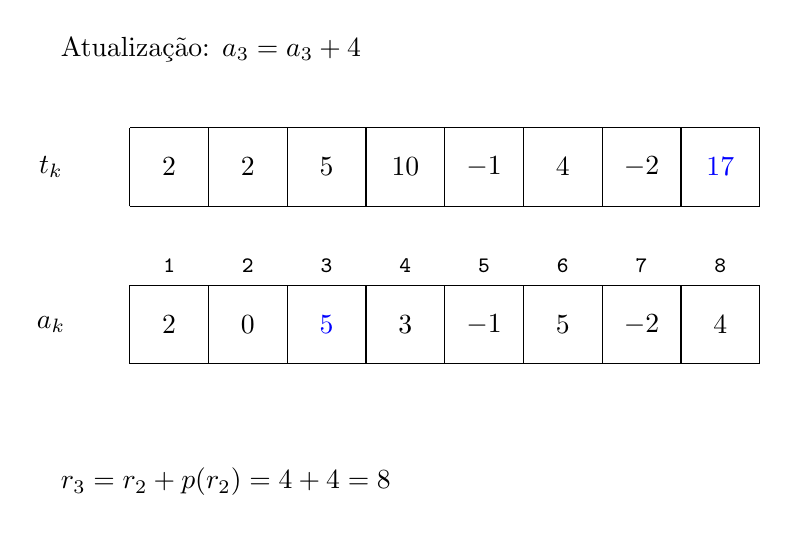
\begin{tikzpicture}
            \node[anchor=west] at (0, 12) { Atualização: $a_3 = a_3 + 4$ };

            \draw (1, 10) grid (9, 11);
            \draw (1, 8) grid (9, 9);

            \node at (0, 8.5) { $a_k$ };
            \node at (0, 10.5) { $t_k$ };

            \node[anchor=west] at (0, 6.5) { $r_3 = r_2 + p(r_2) = 4 + 4 = 8$ };

            \node at (1.5, 9.25) { \footnotesize \tt 1 };
            \node at (2.5, 9.25) { \footnotesize \tt 2 };
            \node at (3.5, 9.25) { \footnotesize \tt 3 };
            \node at (4.5, 9.25) { \footnotesize \tt 4 };
            \node at (5.5, 9.25) { \footnotesize \tt 5 };
            \node at (6.5, 9.25) { \footnotesize \tt 6 };
            \node at (7.5, 9.25) { \footnotesize \tt 7 };
            \node at (8.5, 9.25) { \footnotesize \tt 8 };

            \node at (1.5, 8.5) { \textcolor{black}{$2$} };
            \node at (2.5, 8.5) { \textcolor{black}{$0$} };
            \node at (3.5, 8.5) { \textcolor{blue}{$5$} };
            \node at (4.5, 8.5) { \textcolor{black}{$3$} };
            \node at (5.5, 8.5) { \textcolor{black}{$-1$} };
            \node at (6.5, 8.5) { \textcolor{black}{$5$} };
            \node at (7.5, 8.5) { \textcolor{black}{$-2$} };
            \node at (8.5, 8.5) { \textcolor{black}{$4$} };

            \node at (1.5, 10.5) { \textcolor{black}{$2$} };
            \node at (2.5, 10.5) { \textcolor{black}{$2$} };
            \node at (3.5, 10.5) { \textcolor{black}{$5$} };
            \node at (4.5, 10.5) { \textcolor{black}{$10$} };
            \node at (5.5, 10.5) { \textcolor{black}{$-1$} };
            \node at (6.5, 10.5) { \textcolor{black}{$4$} };
            \node at (7.5, 10.5) { \textcolor{black}{$-2$} };
            \node at (8.5, 10.5) { \textcolor{blue}{$17$} };

        \end{tikzpicture}

    \end{figure}

\end{frame}



\begin{frame}[fragile]{Implementação de {\it update}}
    \inputsnippet{cpp}{43}{63}{codes/segtree.h}
\end{frame}

\section{Implementação {\it top-down}}

\begin{frame}[fragile]{Número arbitrário de nós}

    \begin{itemize}
        \item Na implementação \textit{bottom-up} foi assumido que o tamanho $N$ do vetor
            $xs$ era uma potência de 2

        \item No caso geral, $N$ pode ser um inteiro positivo qualquer

        \item A implementação \textit{top-down} é uma alternativa para estes casos

        \item Se $N$ não é uma potência de 2, a próxima potência de 2 maior do que $N$ é menor
            do que $2N$

        \item Assim uma cota superior segura para o tamanho do vetor $ns$ é de $4N$

        \item O preenchimento de $ns$ é feito por meio de $N$ chamadas de \texttt{update(i, xs[i])}

        \item Este forma não é ótima em termos de complexidade, mas reusa código e diminui o
            tamanho da implementação

    \end{itemize}

\end{frame}

\begin{frame}[fragile]{Implementação do construtor na versão {\it top-down}}
    \inputsnippet{cpp}{1}{18}{codes/segtree_topdown.h}
\end{frame}

\begin{frame}[fragile]{\it Update}

    \begin{itemize}
        \item A atualização deve ser feita por meio de recursão

        \item Os parâmetros da versão recursiva devem ser: o índice do nó atual (\texttt{node}),
            o intervalo que o nó representa (\texttt{[L, R]}), o índice do elemento a ser 
            atualizado em $xs$ (\texttt{i}) e o valor da atualização (\texttt{value})

        \item Há dois casos base: o primeiro acontece se \texttt{i} não pertencer ao intervalo 
            \texttt{[L, R]}, onde a função deve retornar sem fazer nada

        \item Caso contrário, o valor armazenado em \texttt{node} deve ser atualizado usando
            \texttt{value}

        \item Em seguida há o segundo caso base: se \texttt{node} aponta para um folha, a função
            também retorna

        \item As chamadas recursivas repassam a atualização para os filhos à esquerda e à direita
            de \texttt{node}

    \end{itemize}

\end{frame}

\include{update_topdown}

\begin{frame}[fragile]{Implementação de {\it update} na versão {\it top-down}}
    \inputsnippet{cpp}{19}{39}{codes/segtree_topdown.h}
\end{frame}

\begin{frame}[fragile]{\it Range query}

    \begin{itemize}
        \item As \textit{range queries} também podem ser respondidas por meio de recursão

        \item A chamada \texttt{range\_query(a, b)} retorna o valor da operação subjacente em todos
            os elementos de $xs$ cujos índices estão no intervalo $[a, b]$

        \item Para tal, a chamada recursiva deve ter como parâmetros o nó atual (\texttt{node}),
            o intervalo $[L, R]$ que o nó representa e o intervalo $[a, b]$

        \item O primeiro caso base acontece quando $[L, R]\cap [a, b] = \emptyset$, onde a
            função deve retornar o elemento neutro da operação

        \item O segundo caso base acontece quando $[L, R]\subset [a, b]$: neste caso, o valor
            armazenado no nó deve ser retornado

    \end{itemize}

\end{frame}

\begin{frame}[fragile]{\it Range query}

    \begin{itemize}
        \item A chamada recursiva computa a \textit{range\_query} para as subárvores da esquerda
            e da direita, e computa o resultado para o nó a partir destes retornos

        \item A complexidade desta operação é $O(\log N)$

        \item Isto porque, na decomposição 
            \[
                [a, b] = [x_1, y_1]\cap [x_2, y_2]\cap \ldots \cap [x_k, y_k],
            \] 
            onde $[x_i, y_i]$ é um dos intervalos que aparecem na árvore e $[x_i, y_i]\cap
                [x_j, y_j] = \emptyset$ se $i\neq j$, pode haver no máximo um intervalo
                de cada nível da árvore
    \end{itemize}

\end{frame}

\input{range_query}

\begin{frame}[fragile]{Implementação de {\it update} na versão {\it top-down}}
    \inputsnippet{cpp}{41}{61}{codes/segtree_topdown.h}
\end{frame}
